\documentclass[12pt]{article}
\usepackage[margin=1in]{geometry} 
\usepackage{amsmath}
\usepackage{tcolorbox}
\usepackage{amssymb}
\usepackage{amsthm}
\usepackage{lastpage}
\usepackage{fancyhdr}
\usepackage{accents}
\usepackage{graphicx}
\pagestyle{fancy}
\setlength{\headheight}{40pt}

\newenvironment{solution}
  {\renewcommand\qedsymbol{$\blacksquare$}
  \begin{proof}[Solution]}
  {\end{proof}}
\renewcommand\qedsymbol{$\blacksquare$}

\newcommand{\ubar}[1]{\underaccent{\bar}{#1}}

\begin{document}

\lhead{UBC CPSC 425 Computer Vision: Assignment 5} 
\rhead{Winter 1, 2023-24} 
\cfoot{\thepage\ of \pageref{LastPage}}

\subsection*{Stereo Results} The following includes the results of the stereo. \\ 
For stereo, an alpha of $\alpha = -0.01$ gave the minimum EPE of 0.989.

\includegraphics[width=\textwidth]{}
\begin{minipage}{0.49\textwidth}
    \centering
    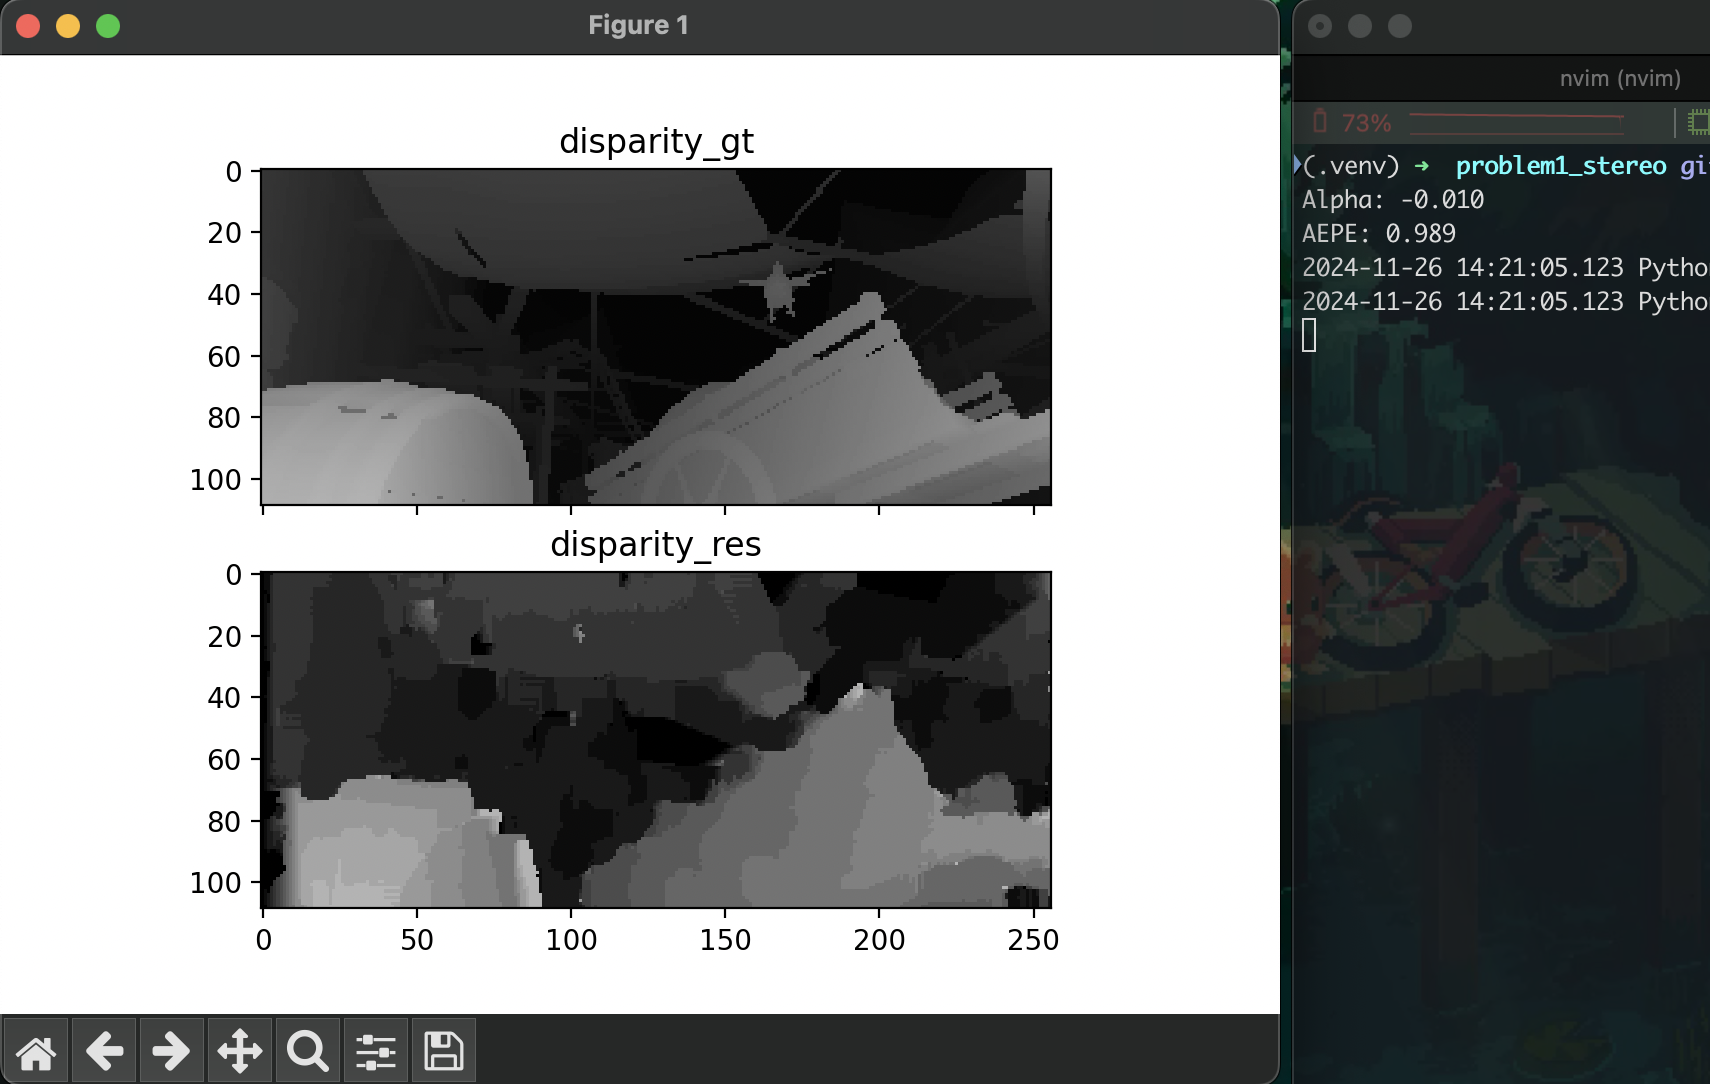
\includegraphics[width=\textwidth]{./problem1_stereo/stereo_results.png}
\end{minipage}
\begin{minipage}{0.49\textwidth}
    \centering
    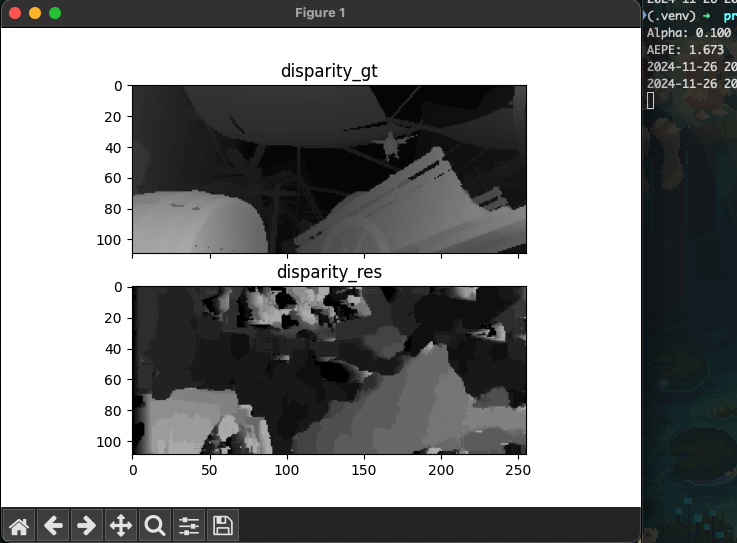
\includegraphics[width=\textwidth]{./problem1_stereo/alpha_0.1.png}
\end{minipage}

\begin{minipage}{0.49\textwidth}
    \centering
    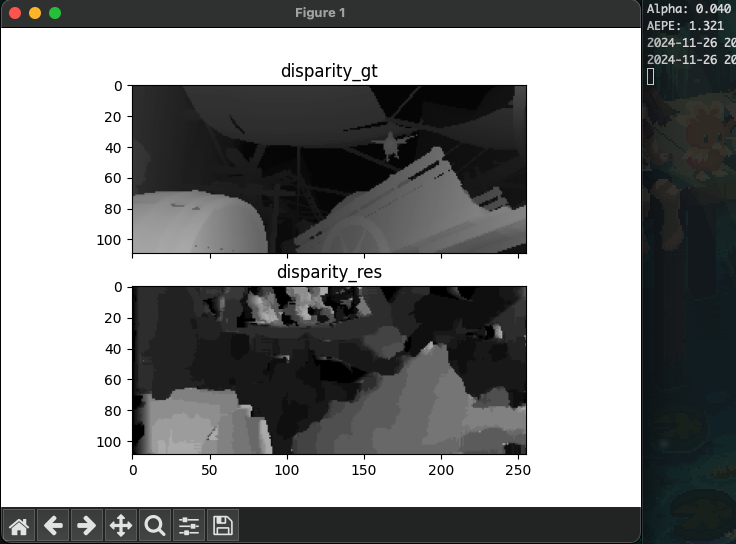
\includegraphics[width=\textwidth]{./problem1_stereo/alpha_0.04.png}
\end{minipage}
\begin{minipage}{0.49\textwidth}
    \centering
    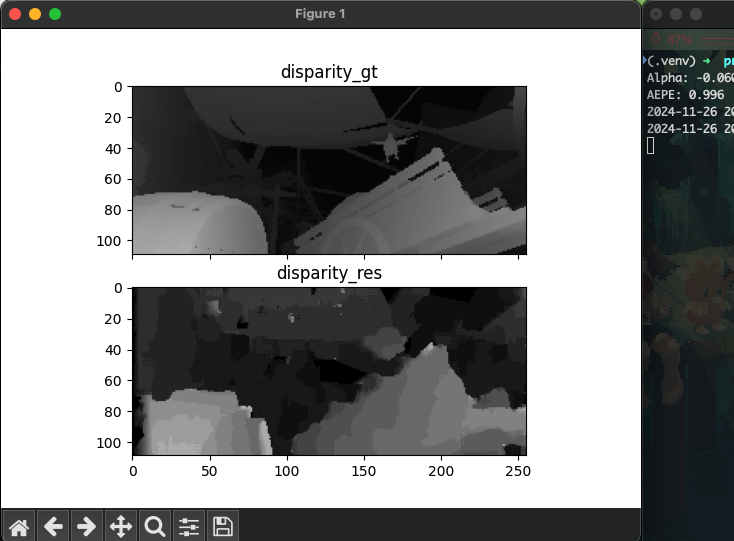
\includegraphics[width=\textwidth]{./problem1_stereo/alpha_neg_0.06.png}
\end{minipage}

\subsection*{Optical Flow Results} The following includes the results of the optical flow. \\ 

\textbf{things: constant}  \\ \\
\begin{minipage}{0.49\textwidth}
    \centering
    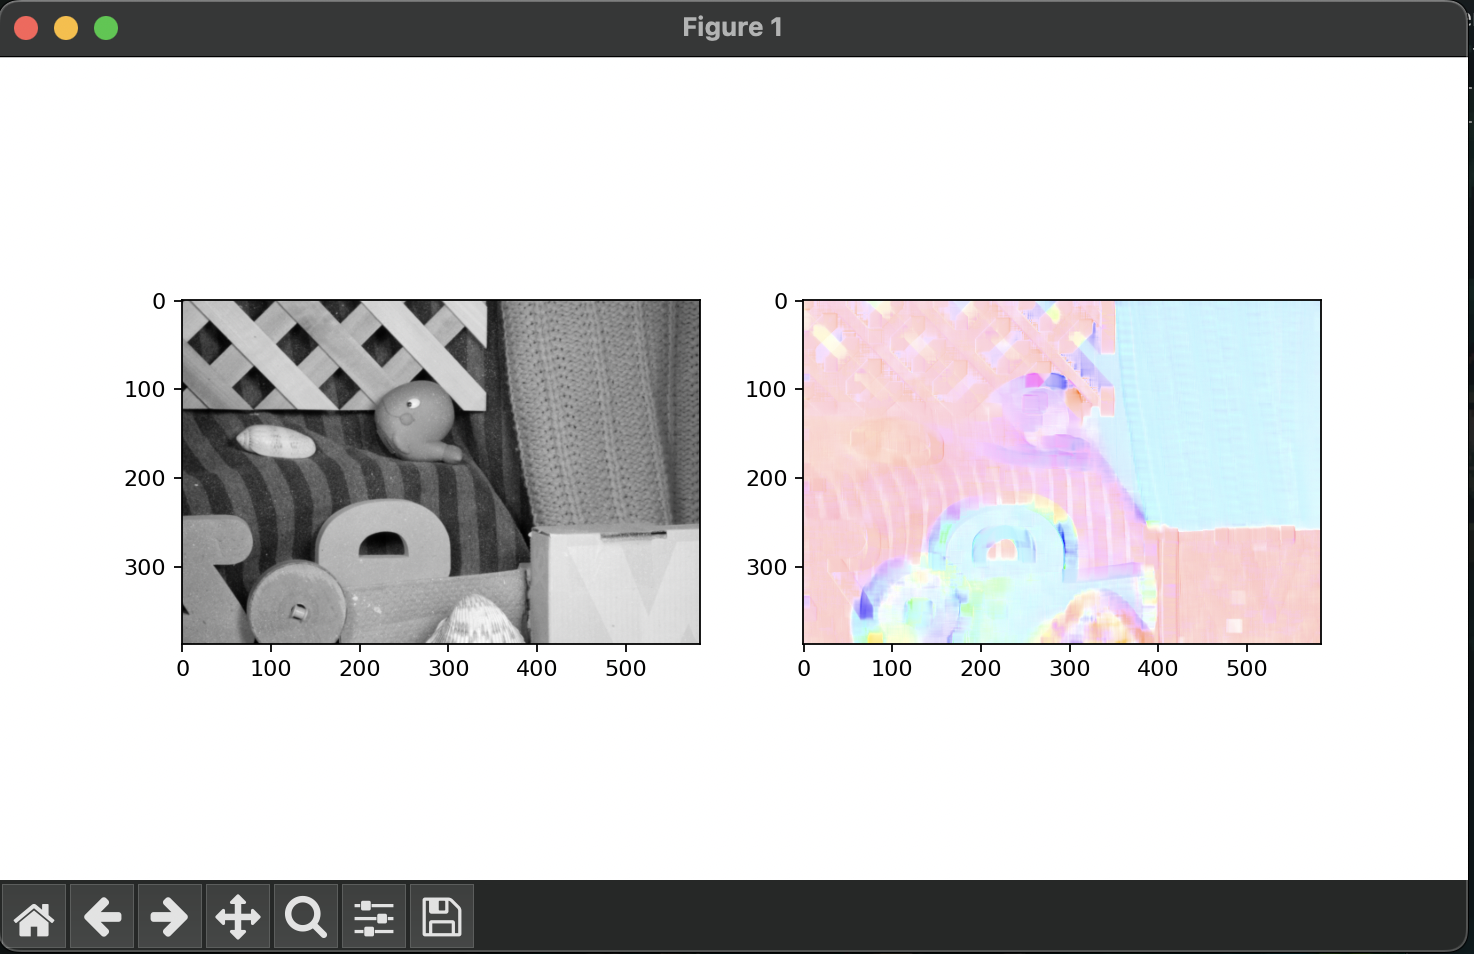
\includegraphics[width=\textwidth]{./problem2_flow/things_constant_image.png}
\end{minipage}
\hfill
\begin{minipage}{0.49\textwidth}
    \centering
    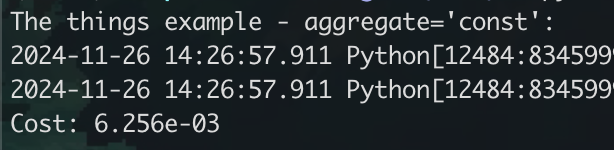
\includegraphics[width=\textwidth]{./problem2_flow/things_constant_result.png}
\end{minipage}

\vspace{1em}

\textbf{things: gaussian} \\ \\
\begin{minipage}{0.49\textwidth}
    \centering
    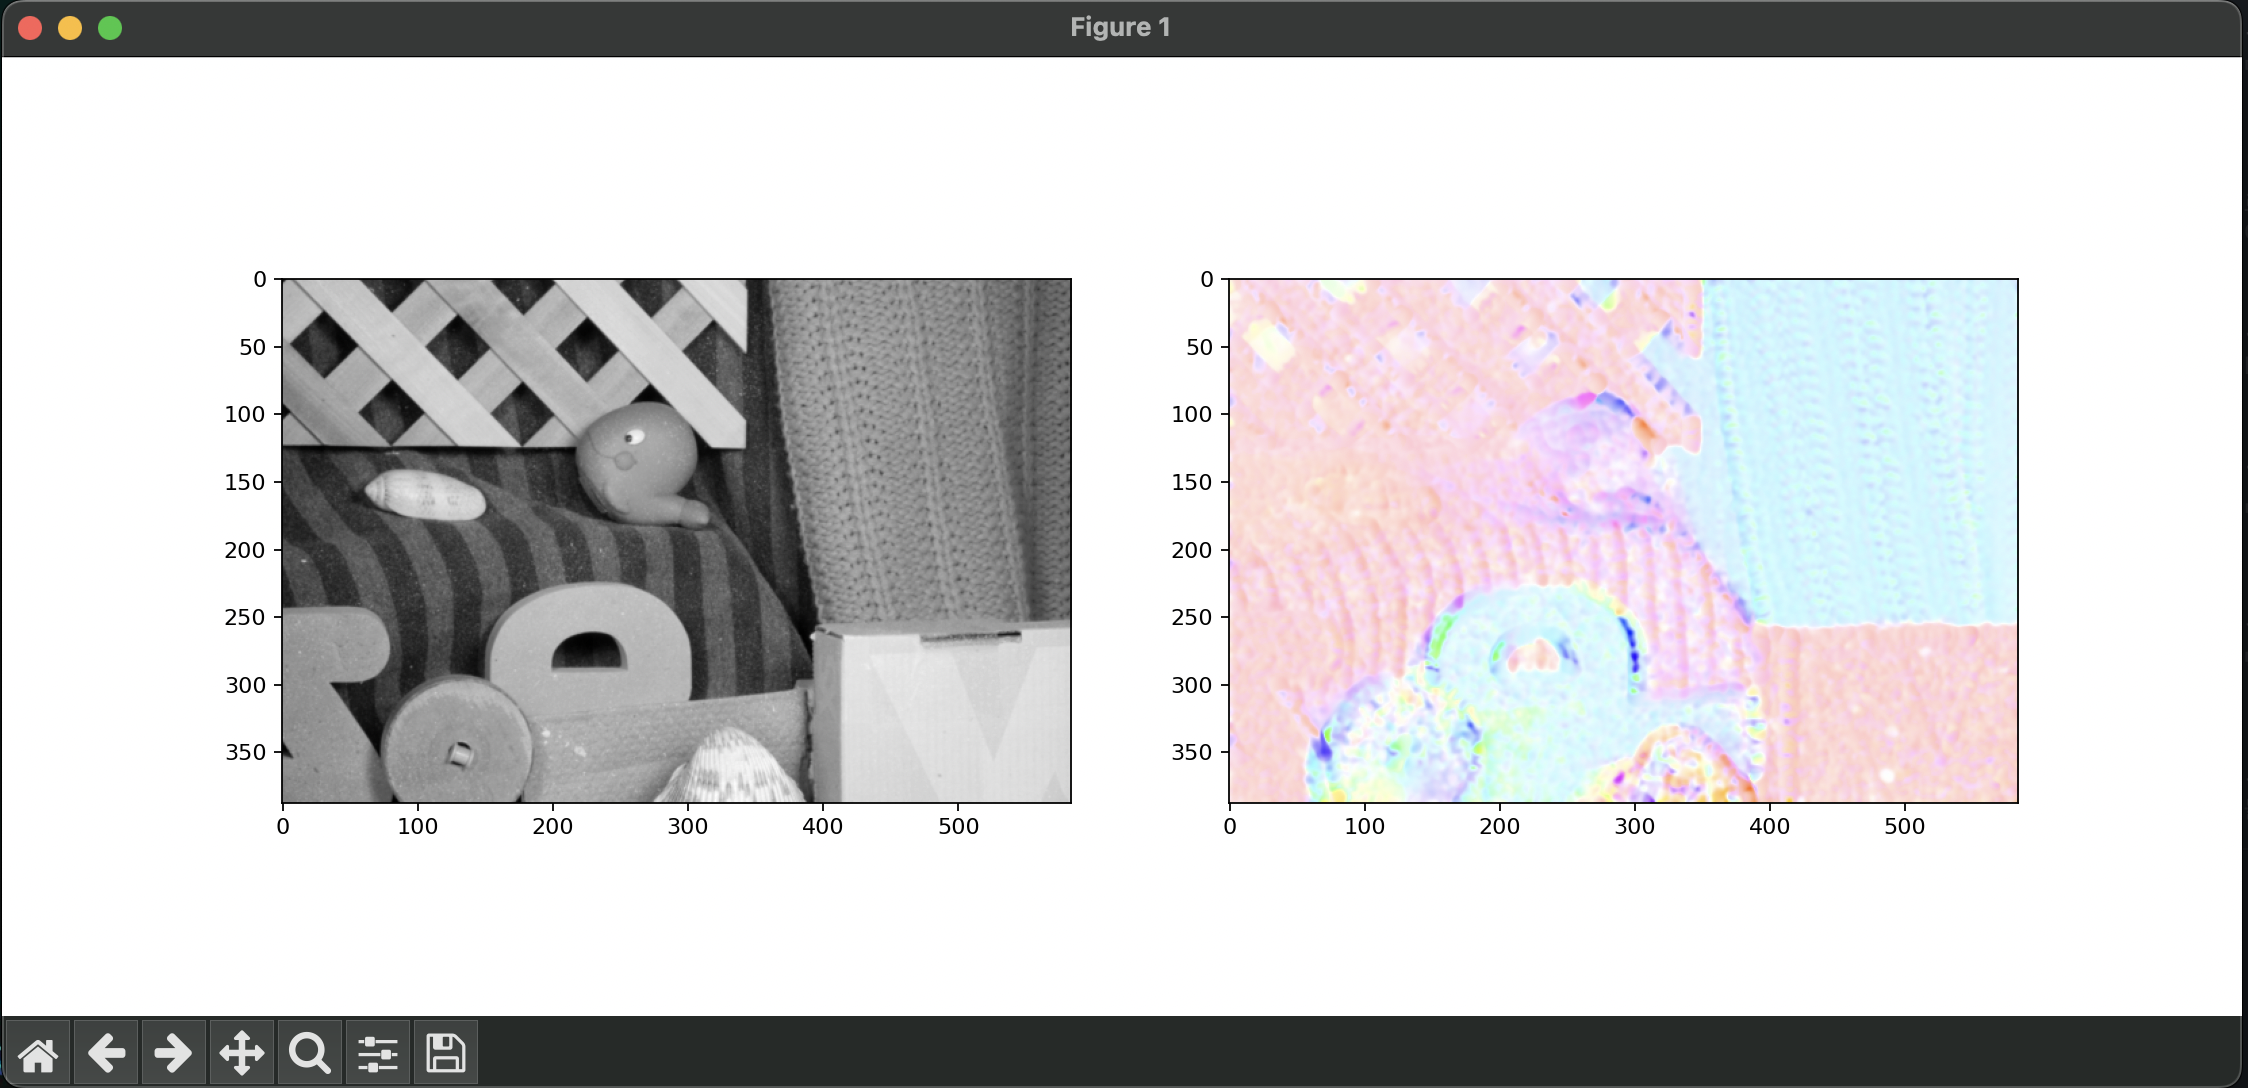
\includegraphics[width=\textwidth]{./problem2_flow/things_gaussian_image.png}
\end{minipage}
\hfill
\begin{minipage}{0.49\textwidth}
    \centering
    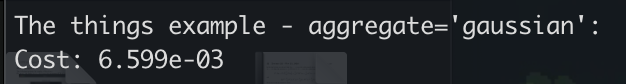
\includegraphics[width=\textwidth]{./problem2_flow/things_gaussian_result.png}
\end{minipage}

\vspace{1em}

\textbf{street: constant} \\ \\
\begin{minipage}{0.49\textwidth}
    \centering
    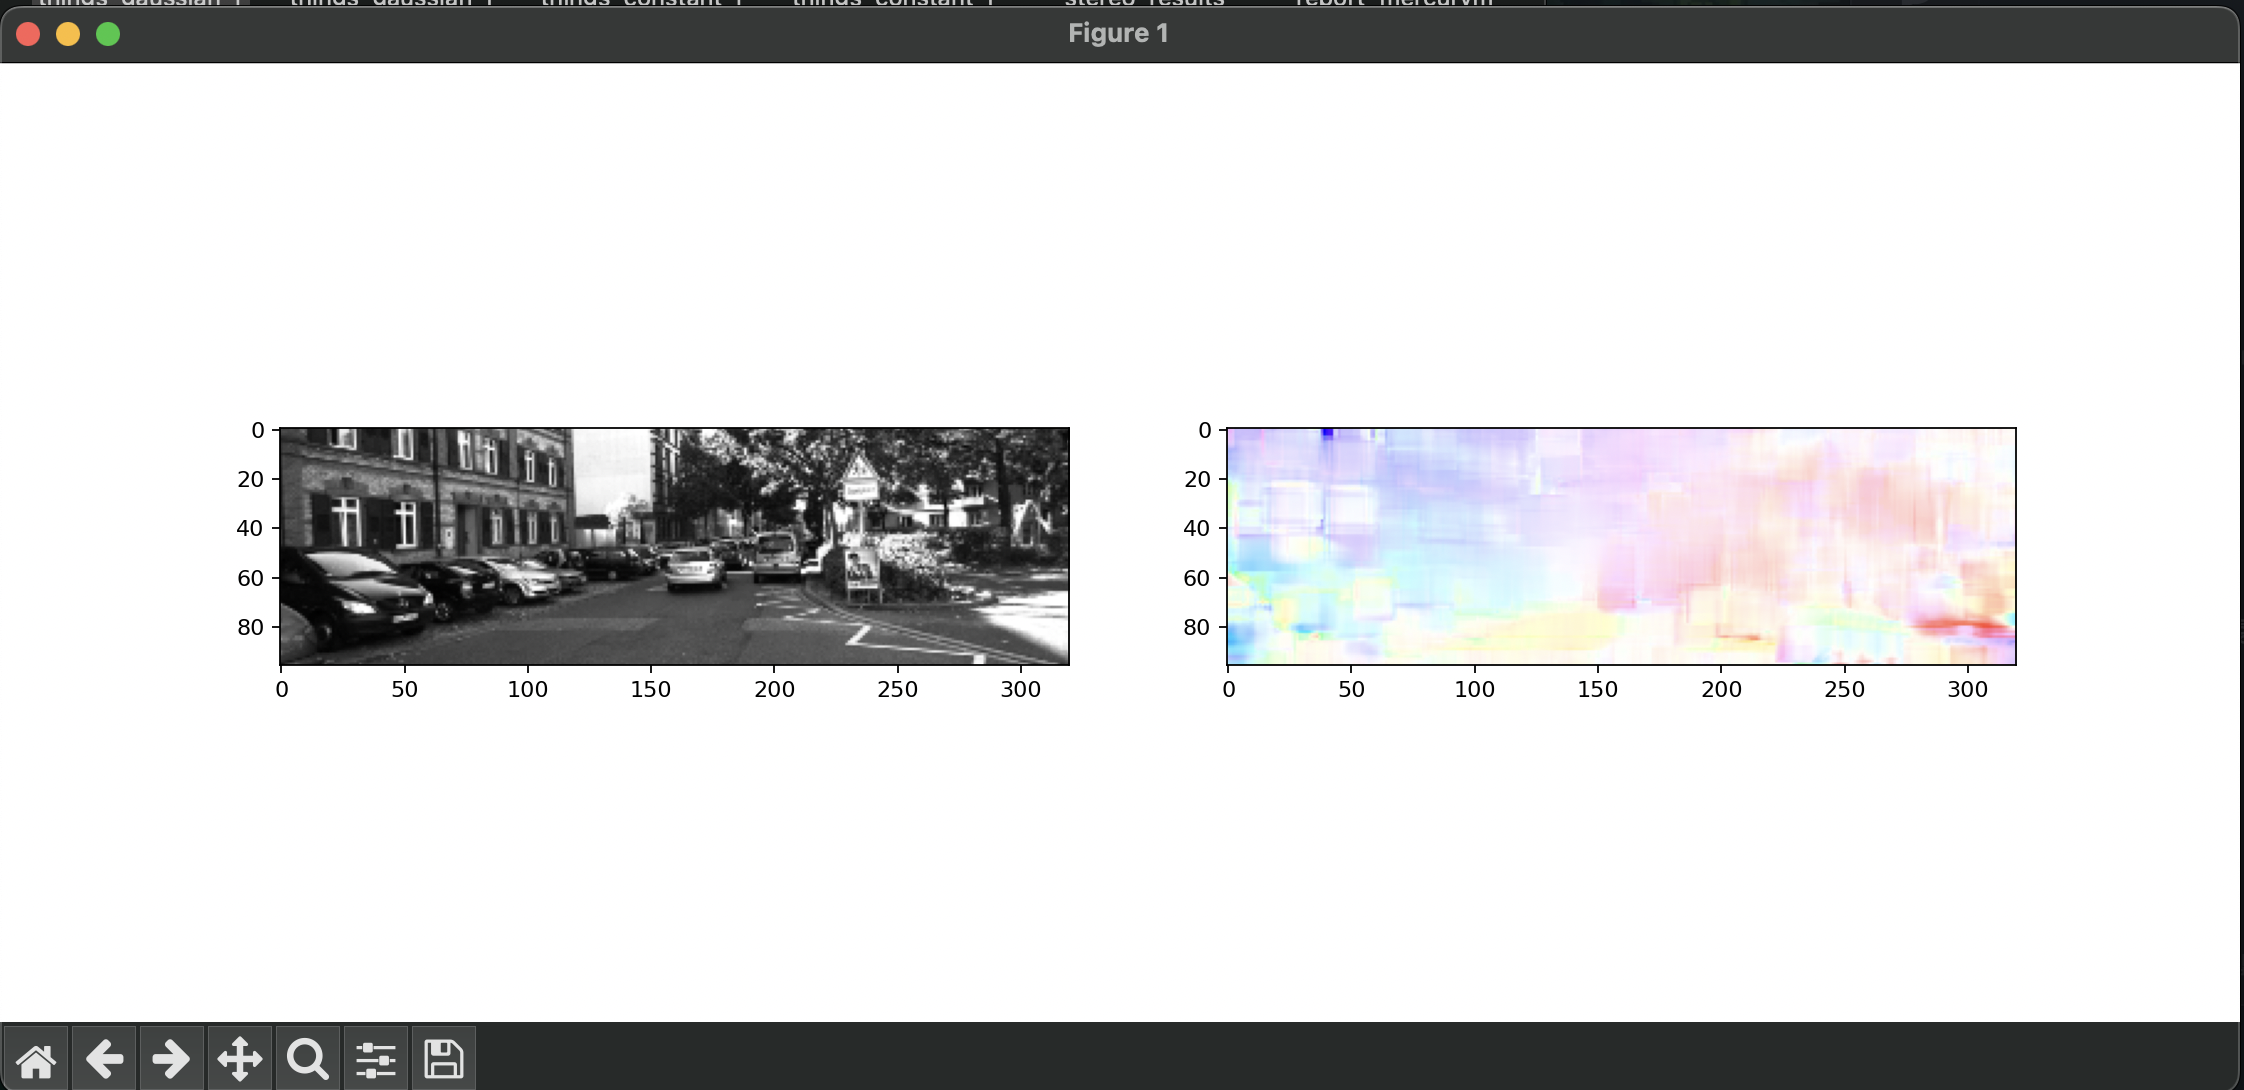
\includegraphics[width=\textwidth]{./problem2_flow/street_constant_image.png}
\end{minipage}
\hfill
\begin{minipage}{0.49\textwidth}
    \centering
    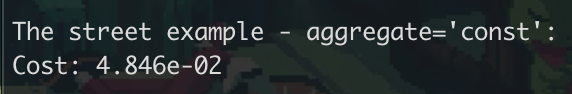
\includegraphics[width=\textwidth]{./problem2_flow/street_constant_result.png}
\end{minipage}

\vspace{1em}

\textbf{street: gaussian} \\ \\
\begin{minipage}{0.49\textwidth}
    \centering
    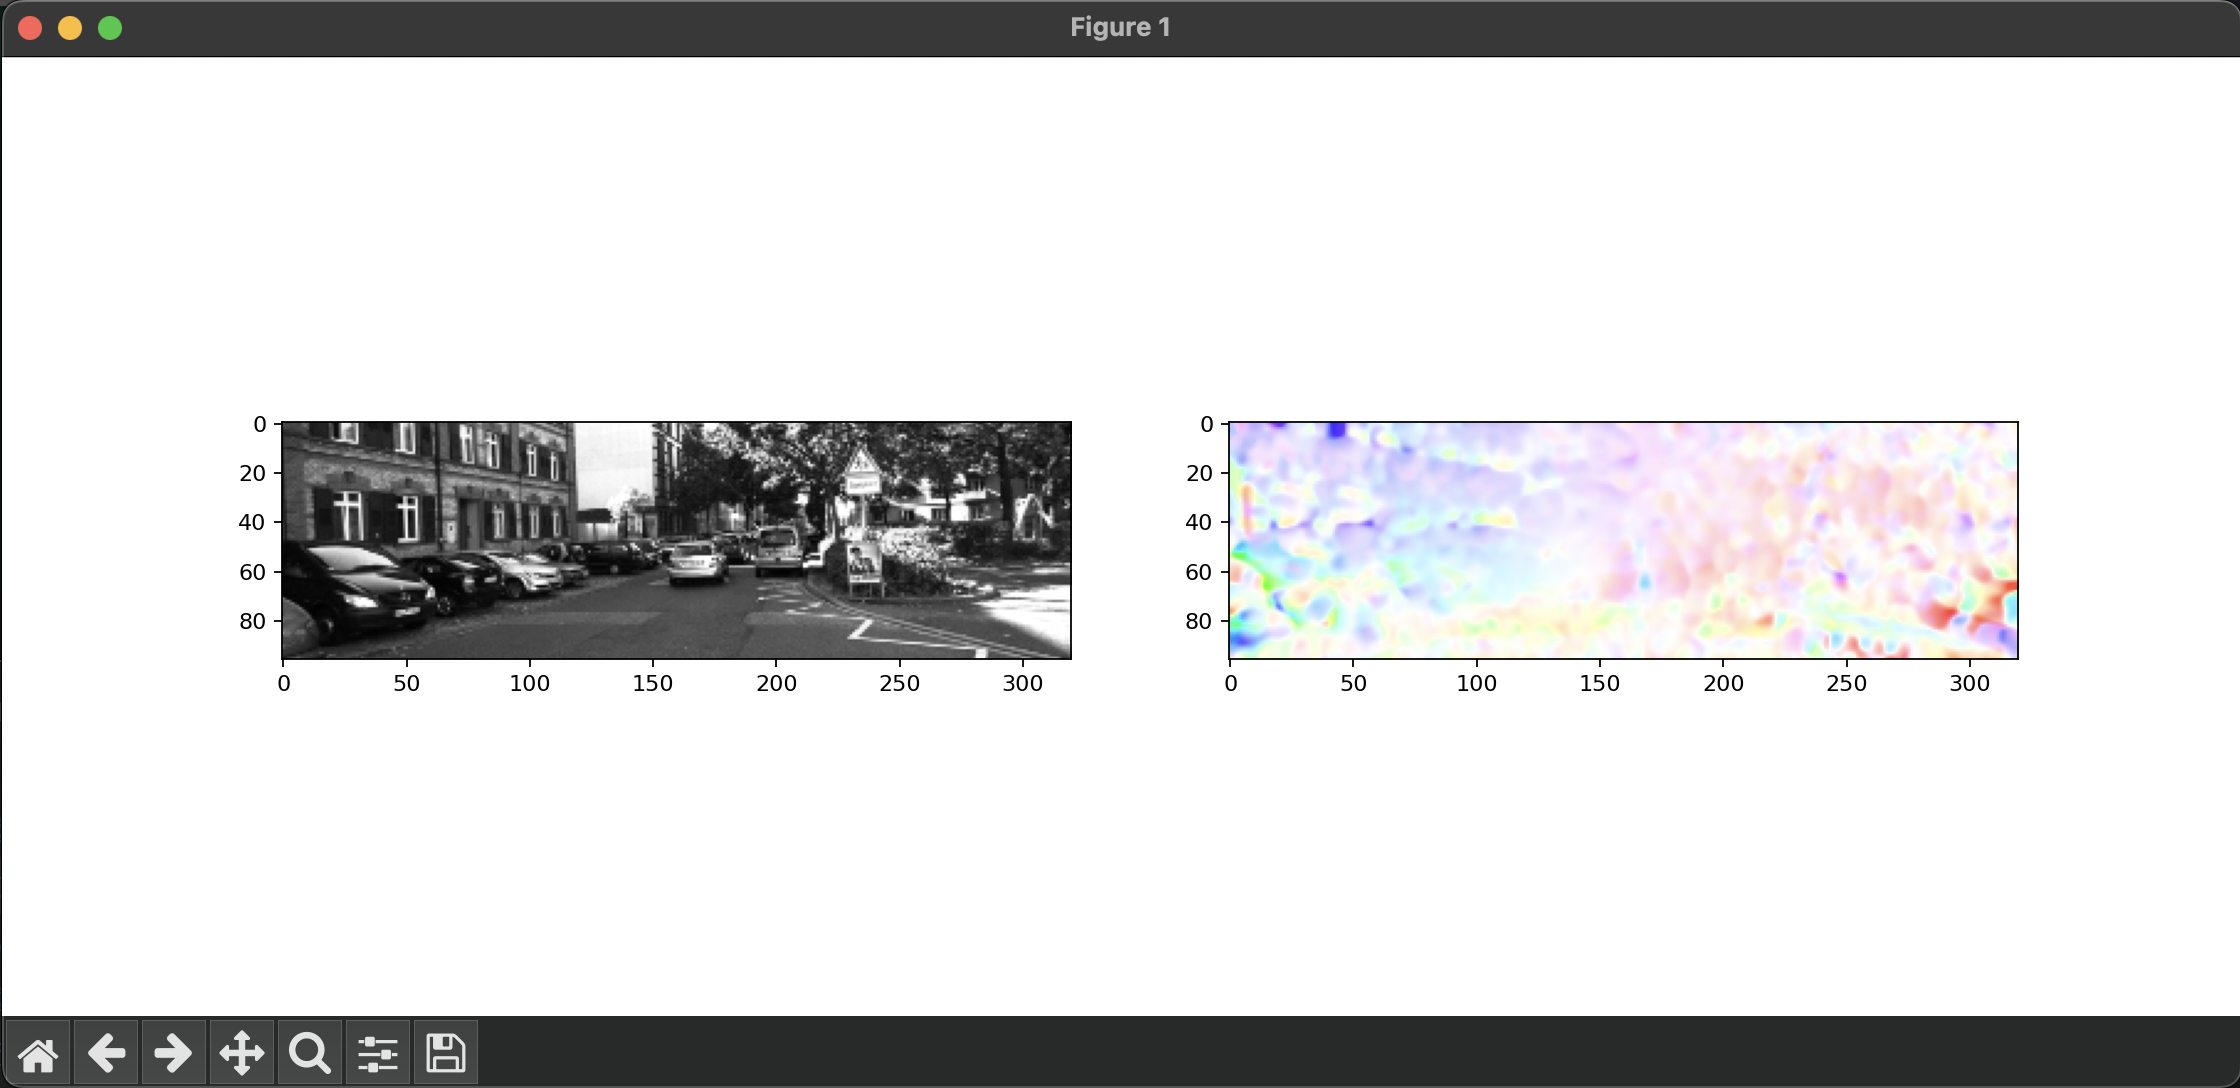
\includegraphics[width=\textwidth]{./problem2_flow/street_gaussian_image.png}
\end{minipage}
\hfill
\begin{minipage}{0.49\textwidth}
    \centering
    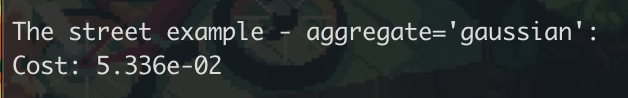
\includegraphics[width=\textwidth]{./problem2_flow/street_gaussian_result.png}
\end{minipage}

\begin{table}[h!]
    \centering
    \begin{tabular}{|l|c|c|}
        \hline
        \textbf{Image} & \textbf{constant} & \textbf{Gaussian} \\ \hline
        Things & 6.256e-03 & 6.599e-03 \\ \hline
        Street & 4.846e-02 & 5.336e-02 \\ \hline
    \end{tabular}
    \caption{Cost Breakdown for Image and Filter}
    \label{tab:costs}
\end{table}

\end{document}
